\label{sec:migration}
In an SDN virtualization infrastructure, the virtual networks are operated by installing flow rules in the underlying physical network.
In the event of a migration, for maintenance purposes or because of an attack, the flow rules will be redeployed on a different physical substrate.

We remind the reader that we limit our study of the migration process to its networking aspect, thus we are not considering the internal specificities of the hypervisors.
We observe the flow rules that will be installed in the SDN nodes by the hypervisor because of the migration, and how the migration can be exploited for unlawful purposes.


\begin{figure}[ht]
\centering
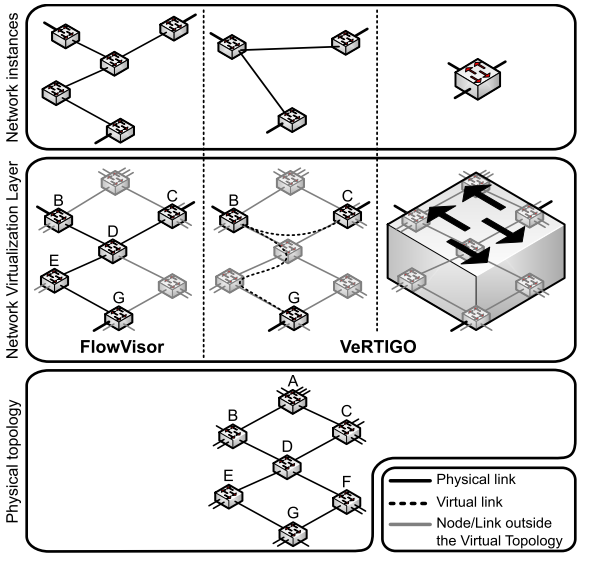
\includegraphics[scale=0.8]{figures/onetomany.png}
\caption{Example of 1-to-many mapping for virtual nodes and links, from VeRTIGO~\cite{VeRTIGO-Corin2012a}}
\label{fig:1tomany}
\end{figure}
\subsubsection{Modeling the migration process}
We have presented in Section~\ref{sec:reference_archi} a reference architecture for the network hypervisor.
From the SDN point of view, a virtual link is a collection of flow rules deployed on one or more physical nodes, to carry the traffic of a specific tenant.
Similarly, a virtual node is the end point of several flow rules.
Therefore, a virtual node can be seen as a collection of flow rules describing the end point of several virtual links on one physical node, SDN-wise.

We include in this work the possibility to describe a one-to-many mapping between a virtual node and a physical node.
Figure~\ref{fig:1tomany} (from VeRTIGO~\cite{VeRTIGO-Corin2012a}) depicts the 1-to-many mapping between virtual and physical elements. Here, the virtual network is composed of three virtual nodes embedded by physical nodes B, C and G.
The virtual link connecting virtual nodes between B and G is seen as a single link while actually there are physical nodes D and E and the corresponding physical links supporting the embedding.
Thus, one virtual link is mapped to many physical resources.

We describe two migration algorithms in the following subsections, a naive algorithm~\cite{Lime-Ghorbani2014} and a more elaborate one~\cite{vnm-lo2013}. 
The ordering of the selection of nodes and links for the migration is studied in~\cite{vnm-lo2013}. 
We consider this to be out of scope of this thesis and we chose a naive ordering for the implementation of the migration algorithms.
We propose our version of the naive algorithm (see Algorithm~\ref{algo:move_algo}) where during the migration phase, both VNs (old and new) will coexist to maintain the availability of the virtual network.


These algorithms use different functions to migrate the topology: create\_link, delete\_link, create\_node, delete\_node and embed. 
Each function will be associated to predicates representing the state of the virtual network during the migration.
We explain what each function does, SDN-wise:

\begin{itemize}
\item Create\_link($vlink\_name,embedding$): This function will deploy flow rules related to $vlink\_name$ on the different nodes composing $embedding$. It generates the $virtual\_link$ and $link\_embedding$ predicates, and returns the identifier of the migrated link.
\item Delete\_link($vlink\_name$): This function will remove the flow rules related to $vlink\_name$ from the physical nodes embedding it.
\item Create\_node($vnode\_name,embedding$): This function will deploy flow rules related to $vnode\_name$ on the different nodes composing $embedding$. It generates $virtual\_node$ and $node\_embedding$ predicates, and returns the identifier of the migrated node.
\item Delete\_node($vnode\_name$): This function will remove the flow rules related to  $vnode\_name$ on the physical nodes embedding it.
\item Embed($vlink\_name \vert vnode\_name$) returns the set of resources allocated for the embedding of either $vlink\_name$ or $vnode\_name$. 
% It is then used to instantiate virtual nodes and links.
\end{itemize}



\subsubsection{Move based migration algorithm}
\label{sec:move-algo}

An intuitive migration algorithm is described in~\cite{Lime-Ghorbani2014}. 
This algorithm aims at migrating the resources all at once.
However, during the migration phase, the VNs are not operational as both are shutdown.
We propose our version of this algorithm (see Algorithm~\ref{algo:move_algo}) where during the migration phase, both VNs (old and new) will coexist to maintain the availability of the virtual network.The underlying aspect of the coexistence of both old and new VNs requires to redirect new incoming flows through the newly migrated VN instead of the old one.
This is handled by setting specific priorities for the flow rules corresponding to the VN.

First (line 3) we initialize $new\_topology$ as the migrated topology. Then, for each virtual node in the topology, we retrieve the new embedding decided by the VNE component (lines 4-5).
Then (line 6) we instantiate the new virtual node and add the information to $new\_topology$.
We repeat the process for the virtual links (lines 7-9).
Then we remove the flow rules related to the old virtual nodes from the original substrate (lines 10-11) and from the old virtual links (lines 12-13).
The virtual network is now completely migrated.




\begin{algorithm}[ht]
\textbf{Input: }$topology$ as the virtual network to be migrated\\
\textbf{Output: } $new\_topology$ as the migrated topology\\
% \State $nodes \gets List\_of\_nodes(topology)$
$new\_topology \gets \emptyset$\\
\For{$node$ \textbf{in} $topology$}{
$embed \gets$ embedding($node$)\\
$new\_topology \gets$~$new\_topology$~$\cup$~create\_node($node$,$embed$)
}
\For{$link$ \textbf{in} $topology$}{
$embed \gets$ embedding($link$)\\
$new\_topology \gets$~$new\_topology$~$\cup$~create\_link($link$,$embed$)
}
\For{$node$ \textbf{in} $topology$}{
delete\_node($node$)
}
\For{$link$ \textbf{in} $topology$}{
delete\_link($link$)
}
\caption{Move based algorithm}
\label{algo:move_algo}
\end{algorithm}


\subsubsection{Iterative migration algorithm}
Another algorithm we consider is described in~\cite{vnm-lo2013}.
This algorithm iteratively moves nodes one after another, while dynamically creating links for the migrated nodes and deleting the old ones.
We represent this algorithm in pseudo-code in Algorithm~\ref{algo:iterative_algo}.
% Create two arrays, one to hold nodes left to be migrated, one to hold the nodes that have been migrated (lines 2-3).

First, we initialize a counter to remember the number of iterations of the algorithm (Line 5).
% While there are nodes to be migrated, do the following (Lines 5 to 28):
Then we select a node among the remaining nodes (line 7), we refer to it as node $n$. We instantiate the new node, referred to as $new\_n$, (line 9) and create the virtual links between the new node and the nodes that have not been migrated (lines 10-14).
If this is not the first iteration of the algorithm, there might be virtual links that must be deployed between the new node and the nodes that have already been migrated. (lines 15-20).
There may also be links between migrated nodes and the old node.
If so, they are deleted (lines 21-24).
We add node $n$ to the list of migrated nodes (line 26) and remove it from the list of nodes that must be migrated (line 27). We finally delete node $n$ (line 28).

We detail the functions used in the following algorithm:
%\GB{again, you are not providing an elaborate explanation with respect to the parameters.}.
%\FC{Done}
\begin{itemize}
\item Select\_node selects the next node to be migrated.
\item exist\_link($node1,node2,topology$) returns True if there is a virtual link between $node1$ and $node2$ in $topology$.
\item link($node1,node2,topology$) returns the identifier of the virtual link connecting $node1$ and $node2$ in $topology$.
\end{itemize}

\begin{algorithm}[ht]
\textbf{Input: }$topology$ as the virtual network\\
\textbf{Output: } $new\_topology$ as the migrated topology\\
 $remaining\_nodes \gets list\_of\_nodes(topology)$\\
 $migrated\_nodes \gets \emptyset$\\
 $iter \gets 1$\\
\While {$remaining\_nodes \neq \emptyset$}{
 $n \gets Select\_node(remaining\_nodes)$\\
 $embed \gets$ embedding($n$)\\
 $new\_n \gets$ create\_node($n,embed$)\\
 \For{$node$ \textbf{in} $remaining\_nodes$}{
    \uIf{exist\_link($new\_n,node,topology$)}{
        $vlink \gets $link($new\_n,node,topology$)\\
        $embed \gets$ embedding($vlink,topology$)\\
        create\_link($vlink,embed$)\\
    }
 }
%  $Deploy\_links(new\_n,remaining\_nodes,topology)$\\
\uIf{$iter>1$}{
%  $Deploy\_links(new\_n,migrated\_nodes,topology)$\\
 \For{$node$ \textbf{in} $migrated\_nodes$}{
    \uIf{exist\_link($new\_n,node,topology$)}{
        $vlink \gets $link($new\_n,node,topology$)\\
        $embed \gets$ embedding($vlink,topology$)\\
        create\_link($vlink,embed$)\\
    }
 }
%  $Deleted\_links(n,migrated\_nodes,topology)$
 \For{$node$ \textbf{in} $migrated\_nodes$}{
    \uIf{exist\_link($new\_n,node,topology$)}{
        $vlink \gets $link($new\_n,node,topology$)\\
        delete\_link($vlink$)
    }
 }
 
 }
 $iter \gets iter + 1$\\
 $migrated\_nodes \gets migrated\_nodes \cup n$\\
 $remaining\_nodes \gets remaining\_nodes / \{n\}$\\
 $delete\_node(n)$\\
 }
\caption{Iterative migration algorithm}
\label{algo:iterative_algo}
\end{algorithm}
